\chapter{Knihovna pro práci s regulárními výrazy}\label{sec:Implementation1}

Před tvorbou samotné vizualizace jsem měl úvahu o použití knihovny, která by mi umožňovala získat zpracovanou strukturu historie průchodu regulárním výrazem.
Sice implementace regulárních výrazů se nachází v samotné specifikaci JavaScriptu,
ale ta mi neumožňuje získat informaci o samotném vyhledávání.
Po prozkoumání existujících řešení, která by vyhovovala této práci, 
jsem se rozhodl vytvořit vlastní implementaci v podobě této knihovny.
Nenalezl jsem totiž řešení, které by bylo dostatečně flexibilní a 
zároveň lehce integrovatelné do programovacího jazyka TypeScript.
Sice vlastní implementace může být pracná, ale jelikož chci mít co nejvyšší kontrolu nad výslednou strukturou, 
tak jsem toto řešení vyhodnotil za vhodné. 

Nejprve v podkapitole~\ref{sec:Imp1LayoutReal} se pokusím vysvětlit návrh této knihovny.
Dále princip parsování regulárních výrazů v podkapitole~\ref{sec:Parse}.
Nakonec v podkapitole~\ref{sec:PatternMatching} popíšu funkčnost vyhledávání s jeho výsledkem.

\section{Architektura}\label{sec:Imp1LayoutReal}

Vstupní třídou pro tuto knihovnu je \textbf{Regexer}. 
Propojuje jednotlivé části této knihovny a také poskytuje její rozhraní.
Dále si drží důležité informace, které souvisí s aktuálně zpracovaným regulárním výrazem.
\textit{RegexMatch} je třída, která reprezentuje jeden výsledek vyhledávání zadaným výrazem.
Její data jsou soukromá, ale umožňuje je procházet pomocí svých metod.
Data této třídy jsou generována třídou \textit{MatchBuilder}.
Její instance existuje pouze ve chvíli, kdy probíhá vyhledávání v zadaném řetězci.
Rozhraní této třídy umožňuje přidávání stavů, které mají v rámci vyhledávání význam informace o aktuálním stavu v regulárním výrazu a hledaném řetězci.
Dále třída \textit{MatcherInternal} má za úkol průchod zadaným řetězcem pro konkrétní výraz.
Tato třída je izolována a není dostupná z vnější, jak její název \textit{internal} (česky vnitřní) napovídá.
Obsahuje hlavní algoritmickou část průchodu nedeterministickým automatem.
Naopak třídou, která poskytuje viditelné rozhraní a volá metody třídy MatcherInternal, je \textit{Matcher}.
Její rozhraní je poskytováno třídě Regexer.
Pro parsování textové reprezentace regulárního výrazu na strukturu NKA a AST, slouží rozhraní \textit{RegexParser}.
Jedná se o parser, který vzniká vždy po překladu bezkontextové gramatiky.
Stack je jednoduchá struktura, která je ale velmi důležitou součástí vyhledávání.
Zásobník programu umožňuje zbavit se rekurzivního volání funkce.
Rekurze obecně vede k pomalejšímu chodu programu a nelze ji jednoduše pozastavit v jakémkoliv čase a stavu.
Také může jednoduše při složitějším zpracování dojít k přetečení zásobníku, který je často limitován, aby nedošlo k nekonečnému rekurzivnímu volání.
Sice rozhraní pole v JS je připraveno na funkcionalitu zásobníku, ale nezaručuje programátorovi striktní pravidla pro zásobník. 
Z tohoto důvodu jsem zvolil jednoduchou implementaci zásobníku, která omezuje manipulaci se základním polem, na operace určené pro zásobník.

Vztahy mezi jednotlivými třídami lze vidět na obrázku~\ref{fig:ARCH_RGXR}. 
Nachází se zde také obalující blok \textbf{MatchingWorker}, který reprezentuje vstupní soubor vedlejšího vlákna, jež slouží pro asynchronní komunikaci s hlavním vláknem.
\textit{Regexer} jako vstupní třída uchovává informace o AST a NKA regulárního výrazu.
Poskytuje také dvě hlavní metody, a to parse pro zpracování výrazu a match pro vyhledání v textu.
Po zavolání metody match se zavolá metoda třídy \textit{Matcher} pro zpracování výrazu.

\begin{figure}[!h]
	\centering
	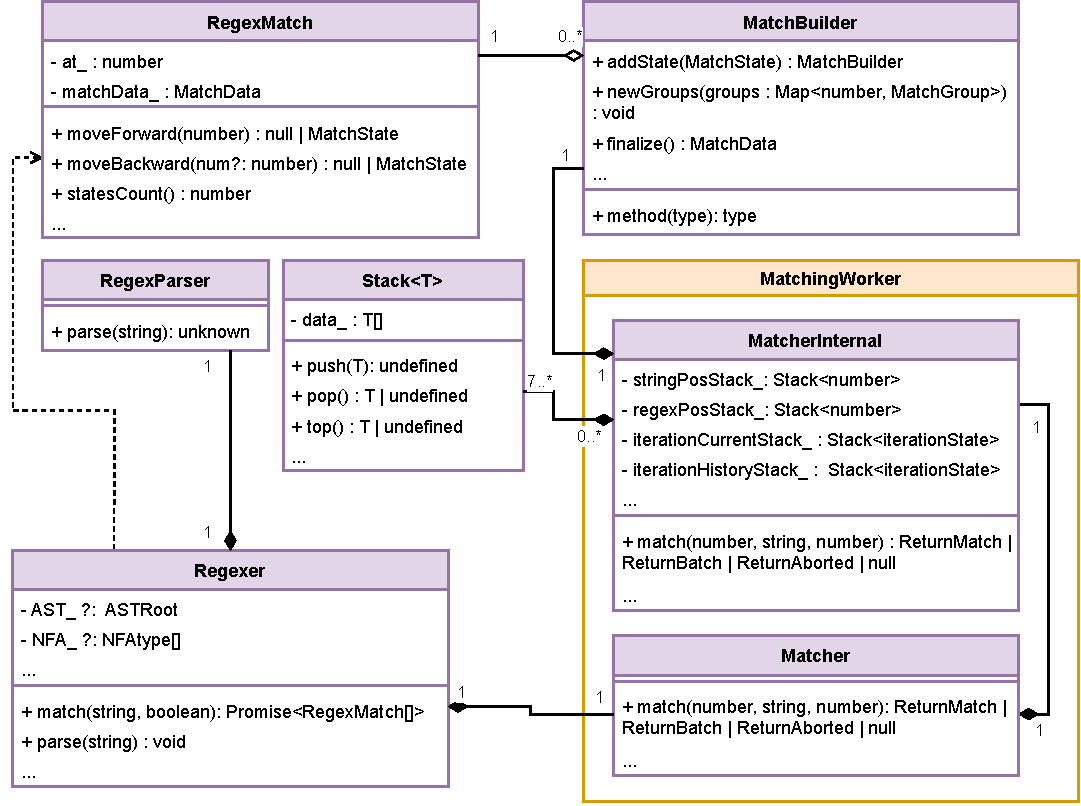
\includegraphics[width=0.9\textwidth]{Figures/UML_RGXR.pdf}
	\caption{Třídní diagram části knihovny pro práci s regulárními výrazy}
	\label{fig:ARCH_RGXR}
\end{figure} 

\section{Parsování regulárních výrazů}\label{sec:Parse}

\subsection*{Parser}

Jak již bylo zmíněno, pro parsování regulárních výrazu jsem použil bezkontextovou gramatiku \textit{Peggy}.
Jedná se o pokračování projektu PegJS, ale ten se již dlouho nevyvíjí. 
Jelikož knihovna Peggy je stále aktualizována a má velkou podporu vývojářů, tak jsem zvolil její využití pro tuto práci.

V ukázce~\ref{code:grammar1} se nachází vstupní neterminál bezkontextové gramatiky \textit{start}. 
Ten obsahuje výběr mezi dvěma začátky \textit{moded\_start} a \textit{general\_start}.
Výběr je pak dostupný pod názvem \textit{type}, podle toho který se zvolí.
Před dokončením pravidla se na jeho konci může nacházet blok "\{\}", který může modifikovat výsledná data.
Modifikace v rámci pravidla pro začátek probíhá zavoláním instance vlastní třídy \textbf{ParserHandler}, která je součástí gramatiky.
Třída má za úkol zpracovávat příchozí data do struktury, která je ukázaná na obrázku~\ref{fig:JSONex}.

\begin{code}[!ht]
	\begin{minted}{peg}
start 
	= 
	type:(moded_start / general_start)
	{
		const data = { modifiers: type?.modifiers };
		return handler.handle(data, type?.elements, States.ROOT);
	}
	\end{minted}
	\caption{Jednoduché pravidlo gramatiky}
	\label{code:grammar1}
\end{code}

Existuje několik různých vzorů regulárních výrazů.
Každý ze vzorů má pravidla pro možné kombinování s ostatními vzory.
Ukázka kódu~\ref{code:grammar2} obsahuje příklad možných výběrů pravidel, které lze společně kombinovat.
Například možnosti pro iteraci, ve zmíněném kódu \textit{to\_iterate}, obsahují pouze následující vzory, které mohou být opakovány.

\begin{itemize}
	\item Speciální znaky (\textit{escaped\_special}) --- "$\textbackslash s$", "$\textbackslash d$"
	\item Základní znaky (\textit{primitive}) --- "$a$", "$b$", "$0$"
	\item Výběr jakéhokoliv znaku (\textit{any\_character}) -- "$.$"
	\item Skupina (\textit{group}) --- "$()$"
	\item List znaků (\textit{list}) --- "$[a-z]$"
\end{itemize}

V mnoha případech záleží na pořadí výběru z dostupných vzorů, proto je potřeba určit, které možnosti upřednostnit.
Abych vysvětlil, proč je pořadí důležité, vybral jsem si jako příklad \textbf{iteraci} (iteration) a \textbf{výběr} (option).
Zjednodušeně výběr má vyšší přednost, jelikož může mít za potomka iteraci.
Kdyby se neterminál iterace nacházel před neterminálem výběru, tak by došlo k tomu, že by iterace nebyla součástí výběru, v případě, že by se nacházela na pozici první možnosti výběru. 
Neboli byla by dříve zpracována, nežli samotný výběr.
Jako příklad může sloužit výraz $a*|b*$, při kterém by se první zpracovala iterace $a*$.
Výsledkem výběru by byly dvě možnosti $\epsilon$ nebo $b*$, což je sice sám o sobě správný tvar výběru, ale ve zvoleném výrazu \textbf{musí} být výsledný výběr $a*$ nebo $b*$.

\begin{code}[!ht]
	\begin{minted}{peg}
any_element 
	= option / iteration / optional / general

to_iterate
	= escaped_special / primitive / any_character / group / list
	\end{minted}
	\caption{Výběry neterminálů pro některé vzory regulárních výrazů}
	\label{code:grammar2}
\end{code}

\subsection*{Struktura zpracovaného regulárního výrazu}

Pro zpracovaný regulární výraz jsem zvolil strukturu, která obsahuje \textbf{nedeterministický konečný automat} (NKA), zároveň s \textbf{abstraktním syntaktickým stromem} (AST).
AST pak slouží k dohledání informací o původním regulárním výrazu. 
Výsledná struktura je objektem, který obsahuje pouze data a má výchozí prototype\footnote{https://developer.mozilla.org/en-US/docs/Learn/JavaScript/Objects/Object\_prototypes}.
Tuto strukturu je možné vidět na obrázku~\ref{fig:JSONex}.
NKA je ve formě \textbf{přesunové tabulky (transition table)}. 
Ta má tvar pole, kde každá položka obsahuje informaci o konkrétním stavu a přesunech na další stavy.
Stav je identifikovaný na základě indexu v poli. 
Přesuny jsou pak implementovány tak, že každý stav si uchovává všechny své přesuny, které vedou z daného stavu do stavu jiného.
Každý přesun pak má informaci, o jaký znak přesunu se jedná a na jaký index (stav) v poli odkazuje. 

Na obrázku~\ref{fig:JSONex} lze vidět výslednou strukturu pro výraz $a+$, která obsahuje dva atributy AST a NFA.
Klíč NFA odkazuje na pole stavů přesunové tabulky. 
AST má odkaz na počátek struktury, který signalizuje začátek regulárního výrazu.
Je zde patrné, že každý stav v tabulce přesunů má odkaz na odpovídající prvek v AST. 
AST prvek/vzor drží různé informace, např. pozice v původním řetězci (start a end), 
potomky daného stavu nebo typ vzoru. 
Ne každý stav musí mít potomky, ale například skupina potomky má.
Některé vzory, jako je například iterace, obsahují v AST dodatečné informace, jako je rozsah iterace (range).
Typy stavů jsou číselné hodnoty, a ty které se nacházejí na obrázku jsou zde také popsány.

\begin{figure}[!h]
	\centering
	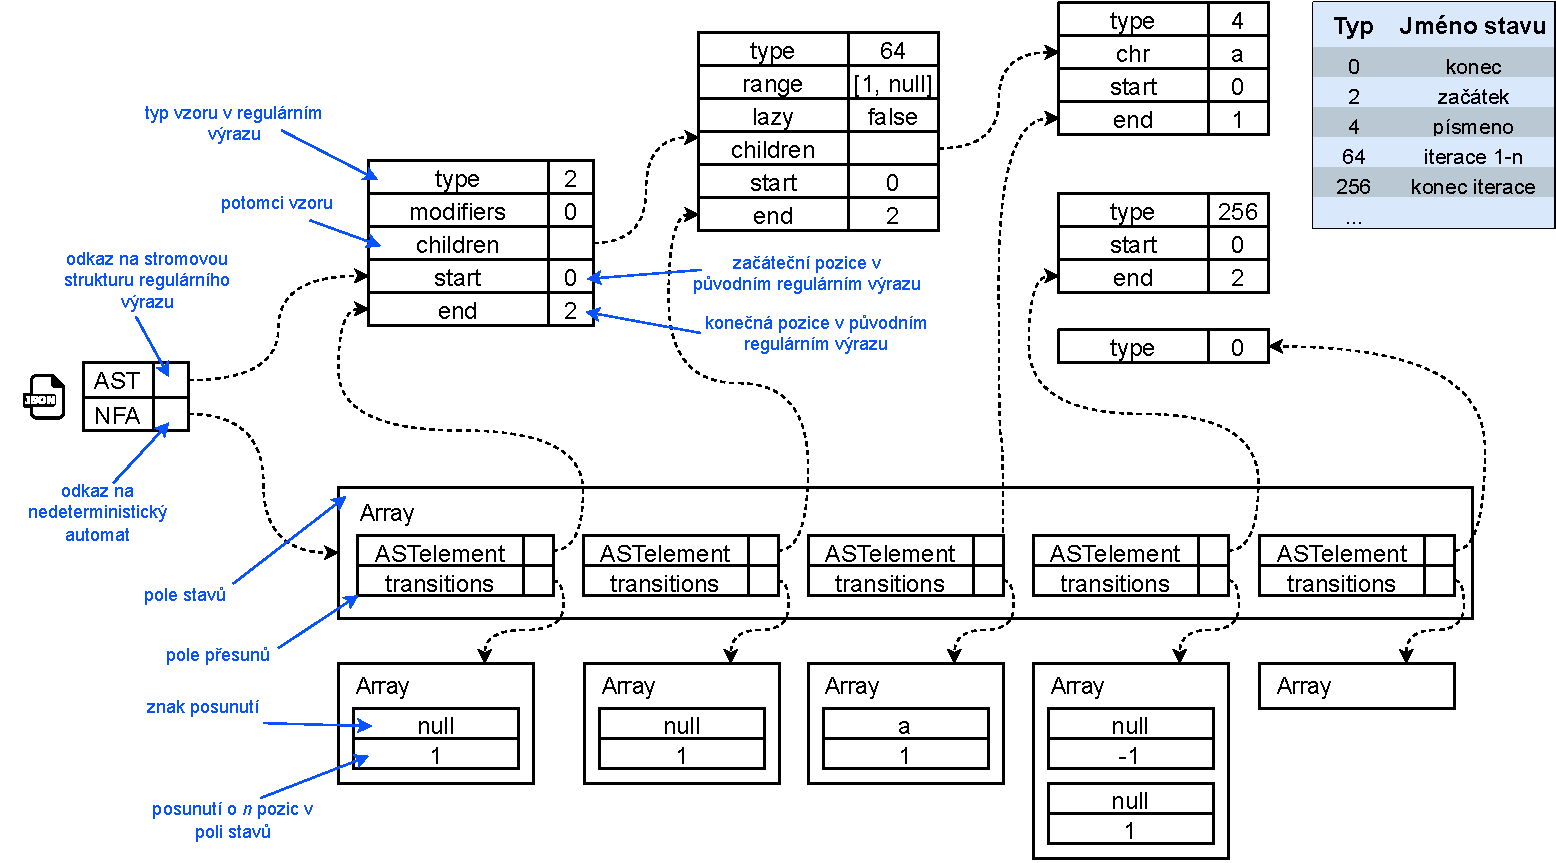
\includegraphics[width=1\textwidth]{Figures/BP-JSON.pdf}
	\caption{Příklad výsledné struktury regulárního výrazu a+}
	\label{fig:JSONex}
\end{figure}

\newpage

\section{Vyhledání pomocí regulárního výrazu}\label{sec:PatternMatching}

Vyhledání je jednou z hlavních částí této knihovny, jedná se o procházení regulárním výrazem a hledaným řetězcem.
Výsledkem je struktura dat, která obsahuje informace o zpracovaném vyhledávání.
V této části textu popisuji, jak jsem naimplementoval vyhledávání, důležité koncepce a výslednou strukturu.

\subsection*{Odstranění rekurze}

Rekurze je sice důležitým aspektem mnoha programů a dokáže usnadnit některé problémy, ale existují situace kdy se vyplatí jí zbavit.
V první řadě bych rád vysvětlil, proč je rekurzivní řešení vhodné pro vyhodnocování regulárních výrazů.
Jak jsem již zmínil, tak v regulárním výrazu může dojít k backtrackingu.
Nastane ve chvíli, kdy není možné z daného stavu v NKA přejít na stav jiný.
V tuto chvíli dojde k vrácení se v NKA do předchozího stavu a k pokračování vyhledávání pomocí další možné cesty.
Nejjednodušší řešení tohoto případu je použití rekurze.
Pro představu, přechod značí rekurzivní volání funkce a pokud není možné přejít do dalšího stavu, tak se vrací do předchozího volání funkce.

Rekurzi lze odstranit pomocí zásobníků, neboli program si uloží jen potřebné informace.
Ve chvíli, kdy dojde k vrácení se (backtrackingu), tak se odstraní vrchol zásobníků.
Důležité tedy je správně řídit správu zásobníků, což může být lehce komplikované.

Úryvek zdrojového kódu~\ref{code:matching1} obsahuje základní vkládání nově navštíveného stavu do zásobníku.
Přesněji se zde ukládá jak stav, tak také index 0 značící počáteční přesun.
Pokud se stav již nachází na vrchu zásobníku, tak je pouze navýšen index přesunu.

% code pushing new state to stack
\begin{code}[!ht]
	\begin{minted}{typescript}
const nfaState = NFA[<number>this.regexPosStack_.top()] as NFAtype;
let topState = this.statesStack_.top();
if(topState?.state !== nfaState)
	this.statesStack_.push({transition: 0, state: nfaState});
else
	topState.transition++;
	\end{minted}
	\caption{Vložení stavu do zásobníku}
	\label{code:matching1}
\end{code}

Příklad kódu~\ref{code:matching2} souvisí s předchozí ukázkou. 
Jestli nastane situace, kdy neexistuje žádný další přesun z aktuálního stavu, je vyvolán backtracking.
Metoda \textit{handleBacktracking} se stará o správu backtrackingu.
Převážně se jedná o odebírání vrchů zásobníků, jako je již zmíněný zásobník stavů.
Pokud není vrácená hodnota \textbf{null}, znamená to ukončení nebo pozastavení vyhledání.
K neúspěšnému vyhledání a následnému ukončení dojde, pokud je zásobník stavů vyprázdněný a pozice v hledaném řetězci se nachází na jeho konci.

% code poping state from stack
\begin{code}[!ht]
	\begin{minted}{typescript}
const transitions = (nfaState as NFAState).transitions;
if(transitions.length <= <number>this.statesStack_.top()?.transition)
{
	const returned = this.handleBacktracking();
	if(returned !== null) return returned;
	continue;
}
	\end{minted}
	\caption{Vyvolání backtrackingu, pokud neexistují další přechody ze současného stavu}
	\label{code:matching2}
\end{code}

\newpage

\subsection*{Počítání iterací a prevence nekonečných cyklů}

Jelikož existují iterace v rozmezí, například od 3 do 6, tak je potřeba znát informaci, v kolikátém opakování se právě konkrétní iterace nachází.
Pro tento problém jsem zvolil osm pravidel, které popisují řešení osmi různých přesunů mezi stavy.
Tato pravidla jsou rozepsána pod obrázkem~\ref{fig:ITERCNT}, indexy pravidel korespondují s indexy v obrázku.


\begin{figure}[!h]
	\centering
	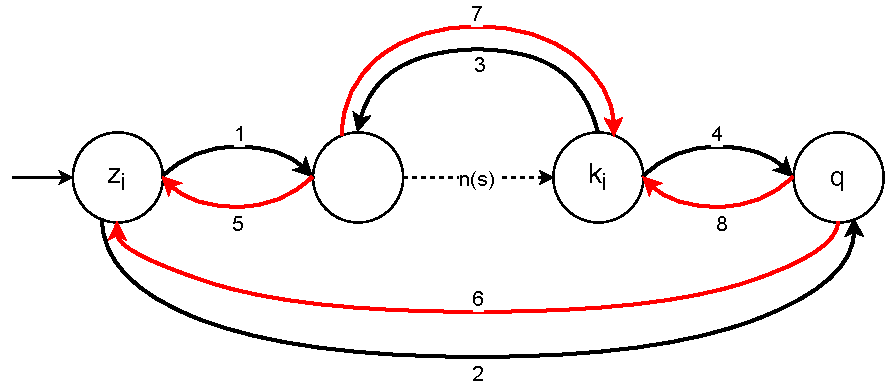
\includegraphics[width=0.65\textwidth]{Figures/IterationCount.pdf}
	\caption{NKA pro popis počítání iterací a prevenci nekonečných cyklů}
	\label{fig:ITERCNT}
\end{figure}

V následujícím seznamu pravidel, $I_i$ značí identifikátor iterace, $i$ je počet dokončených opakování iterace a $P_s$ je aktuální pozice v hledaném řetězci.
$I_{arr}$ obsahuje informace v poli o jedné iteraci [$I_i$, $i$, $P_s$].

\begin{enumerate}[label=\arabic* --]
	\item Vlož do $Z_s$ $\longleftarrow$ [$I_i$, 0, $P_s$]
	\item Vlož do $Z_h$ $\longleftarrow$ [$I_i$, 0, $P_s$]
	\item Vrchol $Z_s$, $I_{arr}$[1] + 1
	\item Vlož do $Z_h$ $\longleftarrow$ Odeber ze $Z_s$, $I_{arr}$[1] + 1
	\item Odeber ze $Z_s$
	\item Odeber ze $Z_h$
	\item Vrchol $Z_s$, $I_{arr}$[1] - 1
	\item Vlož do $Z_s$ $\longleftarrow$ Odeber ze $Z_h$, $I_{arr}$[1] - 1
\end{enumerate}

Na obrázku~\ref{fig:ITERCNT} lze vidět nedeterministický automat. 
Jedná se o obecnou reprezentaci iterace, kde $z_i$ reprezentuje začátek iterace, $k_i$ konec iterace a $q$ značí první stav za iterací.
Mezi $z_i$ a $k_i$ se nachází množina stavů $n(s)$.
Červené šipky signalizují backtracking a černé značí klasický přechod mezi stavy.

Algoritmus pro prevenci nekonečných cyklů a počítání opakování pracuje se dvěma zásobníky určenými pro držení informací o iteracích. 
První uchovává aktuálně nedokončené, resp. probíhající iterace. 
Pro popis jej označuji $Z_s$ (zásobník současných iterací).
Druhý značím jako $Z_h$ (zásobník historie), ten slouží pro iterace, které byly již dokončené.
Historie je důležitá pro backtracking.
Rád bych poukázal na to, že při backtrackingu se vždy zásobníky vrací do původních stavů. 
To znamená, mám-li například stavy $a$ a $b$, tak platí pro přesun $a \rightarrow b$ a pro následující backtracking $b \rightarrow a$, že ve stavu $a$ musí být po dokončení obou přechodů hodnoty zásobníků ve stejném stavu jako na začátku.
Jedno opakování je dokončeno při přechodu 3 nebo 4. 
Zároveň přechod 4 společně s přechodem 2, jsou konečnými přechody pro danou iteraci.

Zásobník současných iterací obsahuje poměrně malé množství informací, jelikož se jedná pouze o probíhající iterace.
Naopak zásobník historie může obsahovat poměrně hodně informací. 
Má-li iterace například 100 dokončených opakování, tak historie bude obsahovat minimálně 100 záznamů.
To se může zdát jako mnoho zbytečných informací, ale nelze předem prakticky vědět jestli dojde k backtrackingu a kde se zastaví.

Další důležitou kontrolou, kterou je nutné splnit, je na konci iterace zkontrolovat zda se nachází v určeném rozmezí.
Jelikož počítám jejich opakování, tak stačí tuto informaci porovnat s náležitými mezemi.

V některých případech by mohlo dojít k nekonečnému cyklu.
Například pro regulární výraz $()+$ by k tomu došlo tak, že by nenastalo k posunu v hledaném řetězci, tím pádem by iterace stále úspěšně procházela dále.
Pro řešení toho problému slouží ukládání poslední pozice v hledaném řetězci při začátku nové iterace nebo zopakování.
Jestli má dojít k zopakování, musí proběhnout kontrola, zdali došlo ke změně pozice v řetězci od posledního zopakování.
V obrázku~\ref{fig:ITERCNT} se jedná o stav $k_i$ a přesun $3$.

\subsection*{Využití vlákna pro vyhledávání}
Nedílnou součástí této knihovny je \textbf{paralelní zpracování} v podobě balíčku Threads.js.
Balíček byl již zmíněn v kapitole~\ref{sec:USEDtech}.
Paralelismus dovoluje složité operace přesunout do vedlejšího vlákna, aby hlavní vlákno nebylo zatěžováno.
Vlákna sice umožňují efektivnější zpracování náročných programů, ale také mají svá úskalí.

V původní formě této knihovny jsem pro samotné vyhledávání použil worker thready, ale později jsem tuto implementaci přepsal s využitím balíčku Threads.js.
Motivací pro tuto změnu byla možnost flexibilnějšího použití, neboli možnost integrace knihovny pro různé runtime.
Tato změna také přinesla značné urychlení vizualizační části aplikace, jelikož vlákno může být spouštěno přímo ve webovém prohlížeči.
Původně toto nebylo možné, jelikož worker thready existují pouze v \textit{NodeJS} runtime.
To znamenalo, že vizualizace závisela na komunikaci s \textit{NodeJS} aplikací, v tomto případě se jednalo o samotné \textit{VSCode} rozšíření.

S volbou vývojového prostředí \textit{VSCode} byla nutnost splnit podmínky stanovené pro práci s web workery, v souladu s jejich API \cite{Microsoft_2021}. 
Podmínkou totiž je, mít zdrojový kód workeru přímo vložený ve zdrojovém kódu hlavního vlákna.
To znamená, že worker nesmí být přímo načítaný z adresáře rozšíření.
Avšak tato podmínka komplikuje samotnou implementaci a proto následovně vysvětlím, jak jsem tento problém řešil.

Všechny závislosti, které worker má, musí být součástí jednoho výsledného souboru.
To je docíleno tím, že přeložím soubor pomocí \textit{webpack}, který vytvoří jeden výsledný soubor.
Pokud by někdo chtěl využít této knihovny v rámci prostředí NodeJS nebo prohlížeče, tak tento překlad probíhá dvakrát pro oba runtime.
Tento soubor může následně být vložen přímo do zdrojového kódu.
Pokud aplikace, která využívá tuto knihovnu, má webpack, může využít loaderu, který jsem pro tuto knihovnu napsal. 
Ten dokáže v místě, kde je worker volaný, vložit jeho zdrojový kód, v rámci textového řetězce.
Výsledkem je worker, který je vložený jako řetězec ve zdrojovém kódu hlavního vlákna.

\subsection*{Výsledek vyhledávání}

Výsledkem vyhledávání je instance třídy obsahující data s informacemi o procházení.
Jejich tvar se neřídí žádným standardem, neboli výsledná struktura je čistě přizpůsobená této práci.
Vlastnosti výsledného objektu obsahují všechny důležité informace.
První hodnotou je, zdali bylo vyhledání úspěšné, či nikoliv. 
Další jsou skupiny, které drží informace, kde se nachází v regulární výrazu a hledaném řetězci. 
Pokud se jedná o pojmenovanou skupinu, tak se také ukládá její jméno. 
Poslední vlastností, která stojí za zmínku, je pole neboli seznam všech po sobě jdoucích stavů.

Ve stavech se nachází údaje, které reprezentují historii průchodu.
Každý stav obsahuje údaj o pozici v řetězci a ve výrazu. 
Také musí být identifikován, o jaký vzor regulárního výrazu se jedná.
Stav může obsahovat další data, která jsou nepovinná, neboli se nenachází ve všech stavech.
Jedná se převážně o typ akce a seznam skupin.
Akce je informace, která upřesňuje typ stavu, jako je například backtracking.
Seznam skupin se může nacházet také v jednotlivých stavech.
Lze pak pozorovat průběh vývoje skupin s vývojem stavů.

Výsledné stavy se mohou lišit, jak dle počtu, nebo také podle tvaru. 
Modifikace vznikne na základě předem určených nastavení.
Ta například umožňují zahodit nežádoucí informace, nebo naopak přidat rozšiřující.
Zvolil jsem tuto možnost nastavení, aby knihovna mohla být univerzálnější a flexibilnější.

Data jsou uložená v objektu, který je dále součástí třídy \textbf{RegexMatch}.
Samotná třída poskytuje pouze rozhraní pro procházení stavů nebo popřípadě pro získání dalších základních informací o vyhledávání.

\endinput